% !TEX root = ../main.tex < 20 pages

% \chapter{Concepts de base du paradigme service Web}
% Une introduction implicite du chapitre %TODO
% Dans ce chapitre on va faire une vue générale sur les technologies
% des services web sémantiques, Pour bien introduire le chapitre
% prochain sur la composition des services web.

\chapter{Les services web: Vue d'ensemble}
Ce chapitre établit une étude du fondement théorique de notre travail
à savoir les concepts de base du paradigme service Web.  Nous
commençons d'abord par présenter un tour d'horizon définissant
l'architecture de référence de ce paradigme ainsi que quelque
définitions proposées dans la littérature. Ensuite nous nous
intéressons à montrer les limitation de l'approche syntaxique de la
description des services web et l'apport de l'enrichissement
sémantique de cette dernière aux processus de la découverte et la
composition des services Web.\\

  % TODO: complete the introduction
\newpage

  \section{Notions de base et technologies associées} 

  Les services Web constituent une approche pour mettre en œuvre le
  paradigme de service, et peut être vue comme une instance de
  l'architecture orienté service.
  
  Dans cette section va parler aussi d'un socle technologique très
  sollicité, On va aussi Détailler l'architecture de base d'un service
  web, ensuite nous introduisons l'architecture étendus.


    \subsection{Définition et caractéristiques }
    Les services Web sont la technologie la plus connue et la plus
    populaire dans le monde industriel et académique pour la mise en place
    d’architectures à services.

    % ARE PROGRAMMABLE COMPONENTS which use the World- Wide-Web as a
    % medium for describing the functionality of real world ser- vices in
    % a computer manipulable way (Kuropka and Nern, 2006)
    Les Web services ont été proposés initialement par IBM
    \cite{kreger2001web} et Microsoft, puis en standardisés par le
    \acrshort{w3c} \footnote{\url{http://www.w3.org/}} et définis
    \cite{WSA} par :\\


    \emph{``Un service web est un système conçu pour permettre
      d'interopérabilité des applications à travers un réseau.  Il est
      caractérisé par un format de description
      interprétable/compréhensible automatiquement par la machine,
      D'autres systèmes peuvent interagir avec le Service Web selon la
      manière prescrite dans sa description et en utilisant des messages
      SOAP, généralement transmis via
      le protocole HTTP et sérialisés en XML et en d'autres standards du Web ''}.\\

    Cette définition surligne les caractéristiques clés de services Web
    \cite{fremantle2002enterprise}:

    \SpecialItem
    \begin{description} % Les caractéristiques des services web Selon la définition de W3C
    \item[Basés sur des protocoles Internet] : L'utilisation de
      \acrshort{http} pour le transport des informations permet de
      traverser les contrôles d'accès dans un environnement hétérogène.
  
    \item[Interopérables] : Le standard \textsc{SOAP} \cite{box2000simple}
      définit comme étant un protocole destiné à l'échange de messages
      structurés véhiculé généralement sur \acrshort{http} et sérialisé en
      \textsc{XML}, permettant le support pour l'interopérabilité.
      
    \item[Basés sur XML] : Le méta-langage de balisage \textsc{XML}
      \textit{eXtensible Markup Language} est un standard Web ouvert par
      \textsc{W3C} \cite{bray1998extensible} offre un cadre standard pour
      la définition de documents Interprétable par des machines.
    \end{description}
    
    M. P. Papazoglou \cite{papazoglou2003service} apporte une autre
    définition de services web:\\
    \emph{``Les services Web sont des éléments auto-descriptifs et
      indépendants des plateformes permettent la composition faible
      coût d’applications distribuées. Les services Web effectuent des
      fonctions allant de simples requêtes des processus métiers
      complexes. Les services Web permettent aux organisations
      d’exposer leurs programmes résultats sur Internet (ou sur un
      intranet) en utilisant des langages (basés sur XML) et des
      protocoles standardisés et de les mettre en œuvre via une
      interface auto-descriptive basée sur des formats standardisés et
      ouverts''}
    % TODO make a comment on this def and introduce the web services
    % composition idea !
    
    
    % TODO organize this mess * Permettre l'interopéabilité des
    % applications, indépendamment des plates-formes et des langages
    
    % * Permettre le couplage faible des applications (évolution
    % indépendante) et leur coopération via des interfaces de haut niveau
    % d'abstraction (services globaux)
    
    % * Permettre une coopération des applications avec un minimum
    % d'intervention humaine
    Curbera et al. \cite{curbera2001web} de ça part proposent la définition suivante :\\
    
    \emph{``Un service Web est une application réseau capable d'interagir
      par le moyen des standards et des protocoles via des interfaces bien
      spécifiés, dans lequel est décris utilisant un langage de
      description fonctionnel
      standardisé''}.\\

    % Brièvement, un service Web est une entité logiciel modulaire,
    % auto-descriptive et autonome accessible via Internet.
    
    \subsection{L'évolution des styles des services web}
    \label{sec:levol-des-styl}

    \input{content/evolution.tex}
    % Les architecture communes des services web SOAP vs REST les limites
    % de la'approche SOAP pourquoi SOAP pour notre problème?
    ``the next section provides a short history of web services, with
    emphasis on the kinds of software challenges that web services are
    meant to address.''
    
    \subsection{L'architecture de référence et technlogies associées}
    \cite{curbera2002unraveling} \cite{gottschalk2002introduction}
    \cite{kreger2001web} \cite{WSA}
    % The basic SOAP/WSDL/UDDI standards are a particular implementation
    % of the concept of a service- oriented architecture.  cette
    % sous-section va détaillé SOAP et pas de WSDL et UDDI
    Cette architecture a été proposée afin de promouvoir
    l’interopérabilité et l’extensibilité des services Web Dans
    l'ensemble, une architecture complète de services Web est
    constitué d'un fournisseur de servicee \footnote{Providers}, un
    annuaire de services \footnote{Service Registry}, et un client
    \footnote{Service Requester} de service.  La figure x montre comment 
    ces trois rôles interagissent.\\

    \SpecialItem
    \begin{description} % TODO tranlate: Les Rôles dans une architecture WSA
    \item[Le fournisseur] A service provider provides the interface for
      the Web service and the implementation of the application. The
      service provider is also responsible for creating the definition of
      the service and publishing that definition to meet the Universal
      Description, Discovery, and Integration (UDDI) specification.
  
    \item[L'annuaire] A service registry is a way in which Web services
      are formally published. The service registry is based on the UDDI
      specification and reflects information about services provided by
      the service provider. The service registry provides a service
      requester with a Web Services Description Language (WSDL) service
      description and a Uniform Resource Locator (URL) that points to the
      service itself.
  
    \item[Le client] A service requester is the consumer of a Web service
      and uses the service registry to gain information about, and access
      to, a Web service.
      
    \end{description}

    For an application to take advantage of Web Services, three behaviors
    must take place: publication of service descriptions, lookup or
    finding of service descriptions, and binding or invoking of services
    based on the service description. These behaviors can occur singly or
    iteratively. In detail, these operations are: \SpecialItem
    \begin{description}% TODO tranlate: WS actions
    \item[Publish] To be accessible, a service description needs to be
      published so that the service requestor can find it. Where it is
      published can vary depending upon the requirements of the
      application (see “Service Publication” for more details).
  
    \item[Find] In the find operation, the service requestor retrieves a
      service description directly or queries the service registry for the
      type of service required (see “Service Discovery” for more
      details). The find operation can be involved in two different
      lifecycle phases for the service requestor: at design time to
      retrieve the service’s interface description for program
      development, and at runtime to retrieve the service’s binding and
      location description for invocation.
      
    \item[Bind] Eventually, a service needs to be invoked. In the bind
      operation the service requestor invokes or initiates an interaction
      with the service at runtime using the binding details in the service
      description to locate, contact and invoke the service.
    \end{description}

    % \begin{description} % SOAP + WSDL + UDDI
    Les services Web sont construits autour de standards qui sont
    \acrshort{soap}, \acrshort{wsdl} et \acrshort{uddi} assurant
    respectivement leur communication, leur description et leur découverte.

      \subsubsection{Communication: SOAP}
      Développé par IBM\footnote{\url{http://www.ibm.com}} et
      Microsoft\footnote{\url{http://www.microsoft.com}}
      \cite{box2000simple}, L'approche \textsc{SOAP} est une recommandation
      \textsc{W3C} qui le définit comme étant un protocole destiné
      à l'échange de messages
      structurés, permettant d'invoquer des applications sur des réseaux
      distribués \cite{mitra2003soap}.\\   
      \begin{figure}[htbp]
    \centering
    \begin{subfigure}[b]{1\textwidth}        
	\centering
	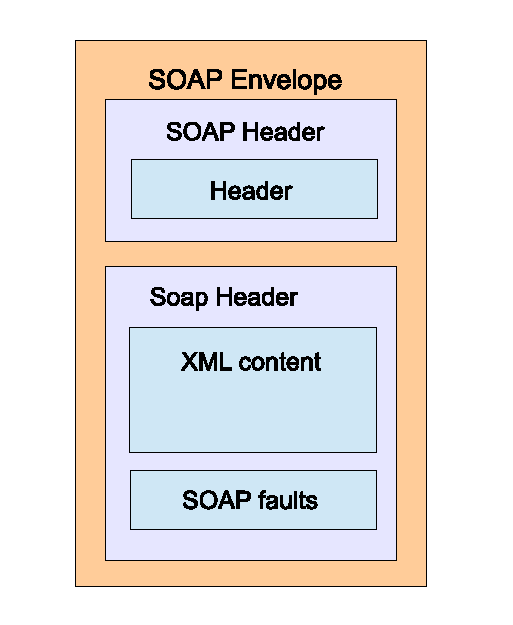
\includegraphics[width=0.5\textwidth]{figs/soap_structure.eps}
	\caption{ Les éléments d'un message \textsc{SOAP}}
	\label{fig:soap_structure}
    \end{subfigure}    

    \begin{subfigure}[b]{1\textwidth}
	\centering
	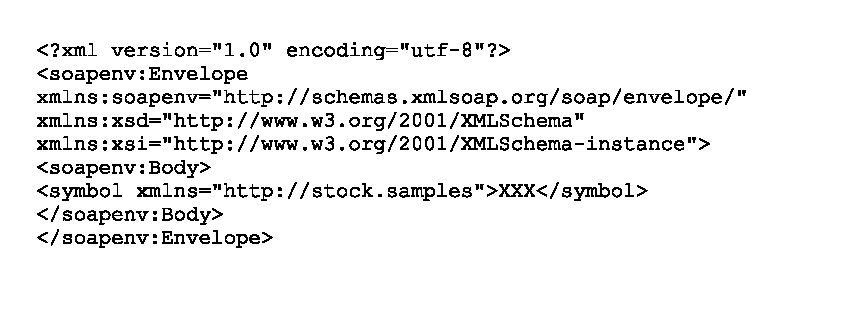
\includegraphics[width=1\textwidth]{figs/soap_message.eps}
	\caption{Exemple de message SOAP}
	\label{fig:soap-message}

    \end{subfigure}
    \caption{La structure d'un message \textsc{SOAP}}
    \label{fig:soap_all}
\end{figure}
 %% La structure d’un message SOAP
      Ce protocole \textsc{SOAP} est basé sur \textsc{XML} pour mettre en place
      un mécanisme valable d'échange des données indépendant du modèle de
      programmation de l'application et du système d’exploitation.
      
      Un message \textsc{SOAP} est un document XML constitué d'une enveloppe
      \textsc{SOAP} obligatoire, d'un en-tête \textsc{SOAP} facultatif et
      d'un corps \textsc{SOAP} obligatoire:

      % TODO pick something real from the app.  go to the annexes part
      % \begin{figure}[h]
    \begin{Verbatim}[frame=single, fontsize=\scriptsize]
	<?xml version="1.0" encoding="utf-8"?>
	<soapenv:Envelope
	xmlns:soapenv="http://schemas.xmlsoap.org/soap/envelope/"
	xmlns:xsd="http://www.w3.org/2001/XMLSchema"
	xmlns:xsi="http://www.w3.org/2001/XMLSchema-instance">
	<soapenv:Body>
	<symbol xmlns="http://stock.samples">XXX</symbol>
	</soapenv:Body>
	</soapenv:Envelope>
    \end{Verbatim}
    \caption{Exemple de message SOAP}
    \label{fig:soap-message-example}
\end{figure}



      % TODO SOAP message structure
      % \begin{figure}
      %   \centering
      % \end{figure}

      \SpecialItem
      \begin{description} % SOAP components
      \item[Enveloppe]: L'élément racine du message \textsc{SOAP} ,
        définissant le contexte du message, son destinataire et son contenu,
        il englobe l'en-tête et le corps.
        
      \item[En-tête \texttt{<Header>}]: Un mécanisme générique permettant
        d'ajouter des fonctions à un message \textsc{SOAP} d'une manière
        modulaire sans accord préalable entre les parties en communication.
        Des exemples d'extension qui peuvent être implémentées comme des
        en-têtes sont des authentifications, des transactions, des paiements
        
      \item[Corps \texttt{<Body>}]: Contient les informations obligatoires
        destinées à l'ultime destinataire du message, il sert comme un
        container pour les informations mandataires à l'intention du
        récepteur du message.  \textsc{SOAP} définit un élément pour le
        corps, qui est l'élément \texttt{<Fault>} (Erreur) utilisé pour
        rapporter les erreurs.
      \end{description}

      \subsubsection{Description: WSDL} %TODO rewrite
      Le langage de description des services Web \acrshort{wsdl}
      \cite{chinnici2007web} est une recommandation du \acrshort{w3c},
      maintenant dans sa deuxième version.  \textsc{WSDL} est basé sur
      \textsc{XML} pour décrire les fonctions opérationnelles de services
      Web. La description des\textsc{WSDL} sont composées d'un interface et
      des implémentations. L'interface est une définition abstraite et
      réutilisable service qui peut être référencée par plusieurs
      implémentations.
      % \begin{figure}[h]
   \begin{Verbatim}[frame=single, fontsize=\small]
	<description>
	    <interface>
		<operation>
		    <input
			messageLabel="xs:NCName"?
			element="union of xs:QName, xs:token"? >
			<documentation />*
		    </input>
		    <output
			messageLabel="xs:NCName"?
			element="union of xs:QName,
			xs:token"? >
			<documentation />*
		    </output>
		</operation>
	    </interface>
	</description>
    \end{Verbatim}

     % \caption{La représentation d'un élément Inteface}
    % \href{http://www.w3.org/TR/wsdl20/#eii-types}
    % \label{fig:wsdl20_interface}
\end{figure}



 TODO WSDL 2.0

      Le WSDL sert à décrire :
      % TODO
      \renewcommand{\labelitemi}{$\bullet$}
      \begin{itemize} % ce que WSDL offrire
      \item le protocole de communication (SOAP RPC ou SOAP orienté message)
      \item le format de messages requis pour communiquer avec ce service
      \item les méthodes que le client peut invoquer
      \item la localisation du service.
      \end{itemize}
      % TODO reference the section

      \subsubsection{Découverte: UDDI}
      \acrshort{uddi} \cite{clement2004uddi} est une standardisation pour la
      publication et la découverte des services Web initialement conçue et
      spécifiée par le Consortium de standards
      OASIS\footnote{\url{https://www.oasis-open.org}}, et il est le
      résultat d'un accord d'un ensemble d’industriels
      Ariba\footnote{\url{http://www.ariba.com/}}, IBM, Microsoft, etc en
      vue de devenir le registre standard de la technologie des services
      Web.

      \textsc{UDDI} complète les technologies basiques de services Web en
      permettant de créer un \textbf{annuaire} permettant de localiser sur
      le réseau le services web recherchés, les services référencés dans
      \textsc{UDDI} sont accessibles par l'intermédiaire du protocole de
      communication \textsc{SOAP}, et la publication des informations
      concernant les fournisseurs et les services doit être spécifiée en
      \textsc{XML} afin que la recherche et l'utilisation soient faites de
      manière \textbf{dynamique} et \textbf{automatique}.

      Un \textsc{UDDI} peut appartenir à un domaine public comme internet ou
      tout autre réseau accessible à un nombre non limité d’utilisateurs,
      comme il peut appartenir à un domaine restreint comme l'intranet d’une
      entreprise ou d'un groupe d'entreprise.
      % TODO UDDI discovery and binding example

      Les données stockés dans l'UDDI sont structurées (en \textsc{XML}) et
      organisées en trois parties connues:

      % TODO
      \begin{description} % les pages d'UDDI
      \item[Pages blanches]: fournissent des descriptions générales sur les
        fournisseurs de services à savoir le nom de l'entreprise qui fournit
        le service, son identificateur commercial, ses adresses, etc.
        
      \item[Pages jaunes]: comportent des descriptions détaillées sur les
        fournisseurs de services catalogués dans les pages blanches d'une de
        façon taxonomique (selon secteurs d'activités par exemple).
        
      \item[Pages vertes]: fournissent des informations techniques sur les
        services Web catalogués. Ces informations incluent la description du
        service, les adresses \textsc{URL}, du processus de son utilisation
        et des protocoles utilisés pour son invocation.
        
      \end{description}
      % TODO talks about:
          % OWL-S and why UDDI approach is semantically poor

      % TODO Conclure cette subsection par la mention du problème de la
      % découverte automatique des services Web et l'insuffisance de la
      % description syntaxique.

  \section{Description des services web}
  % \cite{sivashanmugam2003adding} \cite{mcilraith2003bringing}
  % \cite{vargas2009challenges} \cite{mcilraith2001semantic}
  % \cite{medjahed2004thesis}

  % TODO Refactore and eliminate some repetition TODO get more from
  % \cite{lopez2008selection}
  Une description du service Web est un document par lequel le
  fournisseur de services communique au client les spécifications pour
  invoquer le service Web, Dans cette section nous présentons les
  modèles de description des services web. Nous détaillons dans la
  première sous-section le modèle de description syntaxique
  \acrshort{wsdl} \cite{chinnici2007web} développé et standardisé par le
  \acrshort{w3c} qui est devenu un élément essentiel dans des
  technologies services web. Ensuite en mettant l'accent sur les
  limitations majeurs de cette approche dans un environnement hétérogène
  qui nécessite un certain degré de dynamisité et d'automatisation.
  Finalement, Nous présentons les divers approches sémantiques visant à
  préciser la description d'un service en insistant sur les approches
  d'annotation sémantique et sur les ontologies de services.

    \subsection{Description syntaxique de services}
    % TODO exoend this introduction and give some examples form a real
    % senario
    Le langage de description de services Web \acrshort{wsdl}
    \cite{chinnici2007web} fournit un modèle ainsi qu'un langage basé sur
    \textsc{XML} de description de services Web. Un fichier \textsc{WSDL}
    comprend une description des fonctionnalités d'un service, mais il ne
    se préoccupe pas de l'implantation de celles-ci.  Il contient aussi
    des informations concernant la localisation du service, ainsi que les
    données et les protocoles à utiliser pour l'invoquer. En pratique, le
    document \textsc{WSDL} \footnote{\url{http://www.w3.org/TR/wsdl20/}}
    est un document \textsc{XML} qui se divise en deux parties
    \cite{elie2010} :

    \SpecialItem
    \begin{itemize} % WSDL two main parts
    \item La définition \textbf{abstraite} de l'interface du service avec
      les opérations supportées par le service Web, ainsi que leurs
      paramètres et les types des données.
      
    \item La définition \textbf{concrète} de l'accès au service avec la
      localisation, par une adresse réseau du fournisseur de service
      \footnote{Service Endpoint}, et les protocoles spécifiques d'accès.
    \end{itemize}

    % TODO exemple pratique d'un document WSDL associé avec le document
    % SOAP de la section précédente
    Un document \textsc{WSDL} constitué de quatre éléments principaux
    \cite{chinnici2007web}: \texttt{<Types>}, \texttt{<Interface>},
    \texttt{<Binding>}, \texttt{<Service>}.

    \cite{baryannis2010} \cite{elie2010} \cite{lopez2008selection}
    \renewcommand{\descriptionlabel}[1]{\hspace{1.5cm}\texttt{#1}}
    \begin{description} % WSDL20 elements
      
    \item[<Types>]: L'élément \texttt{Types} sert à un conteneur
      définissant les données figurant dans les messages échangés par le
      service. \textsc{WSDL} supporte des types élémentaires prédéfinis
      (tels que les entiers, les chaînes de caractères et les dates). Si
      les données échangées possèdent une structure particulière, il est
      possible de les décrire à travers un schéma XML \cite{part20012}.
      
    \item[<Interface>]: Les interfaces\textsc{WDSL} offrent une manière
      abstraite de décrire la fonctionnalité du service, Contrairement à
      la représentation concrète offerte par les éléments de
      \texttt{<Bindings>} et de \texttt{<Services>} qui sera décrit plus
      tard.  Une interface \texttt{WSDL} est constitué d'un ensemble
      d'opérations, chacun d'entre eux décrivant d'une simple interaction
      entre le service et le client. Une opération décrit un séquence des
      messages d'entrées/sorties ou un modèle d'échange de message
      \footnote{message exchange pattern} suivie lorsque l'opération est
      invoqué. Pour chaque message contenu dans le motif
      \footnote{pattern}, un type de message est spécifié à l'aide des
      types qui ont été définis précédemment dans le document.
      \textsc{WSDL} contient huit modèles de messages prédéfinis, mais on
      peut facilement définir de nouveaux.
      % TODO refactor this part
    \item[<Binding>]: \cite{elie2010} \cite{baryannis2010} L'élément
      \texttt{Binding} reprend les opérations de l'élément
      \texttt{<Interface>} et leurs associe un protocole de transfert et
      des spécifications des formats de données de message.  La définition
      des protocoles de communication utilisés pour l'invocation du
      service Web permet d'établir le lien, d'une part, entre le document
      et les messages \textsc{SOAP} et d'autre part, entre les messages
      \textsc{SOAP} et les opérations invoquées.

      % A WSDL binding specifies concrete message format and
      % transmission protocol details
      % for an interface. Each operation in a WSDL description must
      % be associated with a
      % binding. Several typical binding extensions are defined in
      % WSDL 2.0 such as SOAP
      % binding or HTML binding, but the service provider is free to
      % use others provided that
      % they are supported by the client and the service
      % toolkits. The syntax for bindings
      % parallels the syntax of interfaces, since each interface
      % construct has a binding counter-
      % part. A binding can either be reusable, meaning that it is
      % applicable to any interface,
      % or not.

    \item[<Service>]: Cet élément définit la localisation du service Web
      décrit. Pour chaque interface décrite, un élément service lui est
      associé. Le sous-élément \texttt{<endpoint>} définit un port d’accès
      en référençant l’élément \texttt{<binding>} associé et en déclarant
      l'\textsc{URL} localisant le service (avec l’attribut
      \texttt{<address>}).

      % A WSDL service element specifies a single interface that the
      % service will support, and
      % a list of endpoint locations where that service can be
      % accessed. Each endpoint must
      % also reference a previously defined binding to indicate what
      % protocols and transmis-
      % sion formats are to be used at that endpoint. A service is
      % only permitted to have
      % one interface but there are workarounds for a service to be
      % able to expose multiple

      % précise l’adresse ou les adresses aux-quelles se trouve le
      % service. Un <service> est un ensemble
      % de <port>. Un <port> spécifie une adresse pour un <binding>
      % donné. Par exemple

      % Cet élément définit la localisation du service Web
      % décrit. Pour chaque
      % interface décrite, un élément service lui est associé. Le
      % sous-élément endpoint définit un
      % port d’accès en référençant l’élément binding associé et en
      % déclarant l’URL localisant le
      % service (avec l’attribut address). Ceci permet qu’une
      % interface d’un service possède plus d’une
      % localisation (i.e. plus d’un élément endpoint) pour répondre
      % aux problèmes d’indisponibilité.
    \end{description}

    \subsection{Ajout de la sémantique}
    % Pour pallier le manque de sémantique de WSDL, plusieurs approches
    % proposent de rajouter une couche au dessus de WSDL complétant la
    % description syntaxique par des précisions sémantiques.
    % \cite{lopez2008selection}
    Malgré les améliorations apportées au standard \textsc{WSDL} dans son
    deuxième version \cite{chinnici2007web}, la description du service
    reste uniquement au niveau fonctionnel, c'est-à-dire qu'elle contient
    la manière dont on peut utiliser le service et non ce que fait le
    service, le standard \textsc{WSDL} est limité à l'énumération des
    opérations et à la description des types des paramètres d'entrée et de
    sortie associés, elle ne caractérise pas la sémantique de la
    fonctionnalité accomplie par le service. Par conséquent, la
    description \textsc{WSDL} reste insuffisante lors du processus de
    sélection.  Pour pallier cette Difficulté, plusieurs approches
    proposent de rajouter une couche au dessus sémantique de \textsc{WSDL}
    complétant la description syntaxique par
    des précisions sémantiques.\\
    % explain the problem in the context if web services composition using
    % ...  \cite{bartalos2011effective}

    Dans un premier temps, on va essayer de clarifier la notion d'un
    services Web sémantique, puis étudie les langages émergeants qui
    permettent de décrire ce type de services Web.

      \subsubsection{Définition des services Web sémantiques}
      % TODO the semantic web stack in the appendix

      % la description syntaxique est insuffisante.  A Semantic Web service
      % is defined as an extension of Web service description through the
      % Semantic Web annotations, created in order to facilitate the
      % automation of service interactions . Therefore, from he perspective
      % of the functionality offered, Semantic Web services are still Web
      % services. The only difference lays in their description and the
      % consequent benefits that follow, namely the reduction of human
      % involvement in
      % he performed interactions.\\

      % What is semantic web?

      % Le Web tel que nous le connaissons aujourd'hui est encore conforme à
      % la vision initial

      % Le Web a été conçu principalement pour une utilisation par les
      % humains. Néanmoins, il existe un effort visant à automatiser son
      % utilisation et pour apporter le Web plus accessible pour les
      % machines

      % \cite{bartalos2011effective} The Web was primarily designed for use
      % by humans. Nevertheless, there is an ef- fort to automate its use
      % and bring the Web more accessible for machines. This has brought
      % forward the need for machine processable representations of
      % semantically rich information. This has brought forward the need for
      % machine processable representations of semantically rich
      % information: a vision at the heart of the Semantic Web

      L'objectif premier du Web sémantique est de définir et lier les
      ressources du Web afin de simplifier leur utilisation, leur
      découverte, leur intégration et leur réutilisation dans le plus grand
      nombre d'applications \cite{berners2001semantic}. Le Web sémantique
      doit fournir l'accès à ces ressources par l'intermédiaire de
      descriptions sémantiques exploitables et compréhensibles par des
      machines. En effet, Les technologies du Web sémantique complètent le
      Web actuel avec des outils sémantiques. Il ne s'agit donc pas de créer
      un nouveau Web ou un Web séparé de l'existant : ce Web de données
      repose entièrement sur les technologies et concepts qui ont fait le
      succès du Web tel que nous le connaissons aujourd'hui
      \cite{bertails2010web}.

      La réalisation du Web sémantique trouve ces racines dans le
      développement des langages de balisage inspiré par des travaux issue
      de la communié AI \cite{mcilraith2001semantic}, tels que \textsc{OIL}
      \cite{fensel2001oil}, \textsc{DAML+OIL} \cite{horrocks2002daml+oil} et
      \textsc{DAML+OTN} \cite{mcguinness2003daml} (ces deux derniers
      langages sont parties de la famille \acrshort{daml}).

      % TODO refactor
      Ces langaes ont une sémantique bien définies et permettent le balisage
      et la manipulation des taxonomique complexe et Des relations logiques
      entre les entités sur le Web. \cite{fensel2000creating}

      %!TEX root = ../main.tex
\begin{figure}[h]
    \centering
    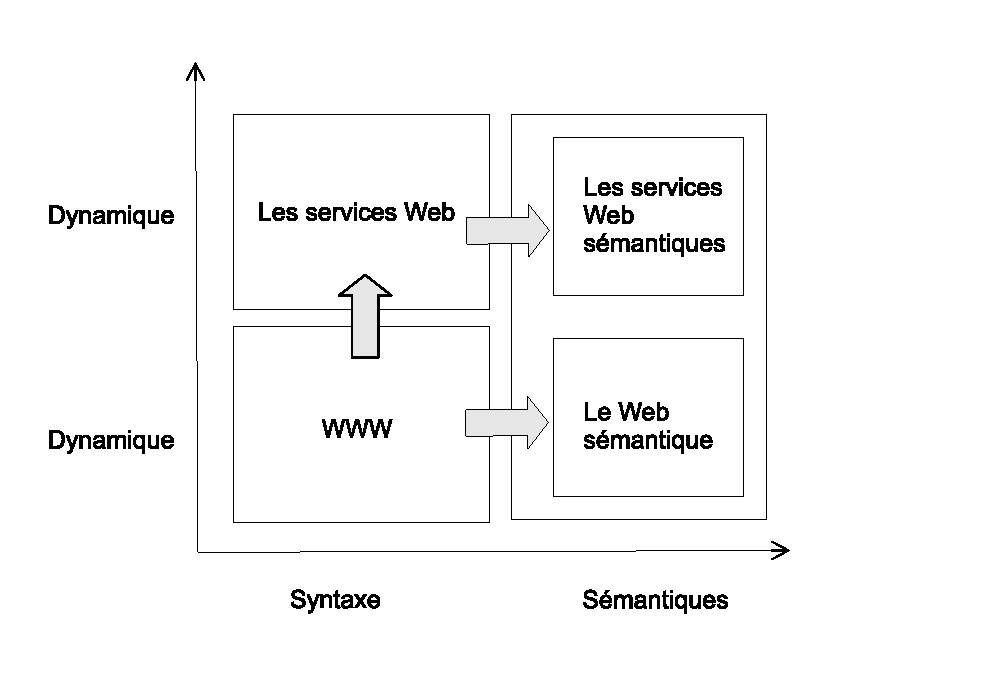
\includegraphics[width=1\textwidth]{figs/3w_to_sws.eps}
    %TODO translate
    \caption{Web evolution to Semantic Web services \cite{fensel2002semantic}.}
    \label{fig:3w_to_sws}
\end{figure}
      % \cite{lopez2008selection}
      Cette description repose sur des ontologies. Selon Gruber
      \cite{gruber1993translation}, une ontologie est une spécification
      explicite d'une conceptualisation. Une conceptualisation est un modèle
      abstrait qui représente la manière dont les personnes conçoivent les
      choses réelles dans le monde et une spécification explicite signifie
      que les concepts et les relations d'un modèle abstrait reçoivent des
      noms et des définitions explicites. Le Web sémantique est devenu un
      domaine à part entière, preuve en est la création en 2001 du groupe de
      travail sur ce sujet par le \textsc{W3C}.


      %  % Semantic web services
      % \cite{fensel2001oil}

      % What I need here ?  the base \cite{lopez2008selection}

      % \cite{berners2001semantic} % semantic web
      % \cite{bray1998extensible} % XML
      % \cite{part20012} % XML schema
      % \cite{lassila1999resource} %RDF
      % \cite{brickley2000resource} % RDFS
      % \cite{mcguinness2004owl} % OWL
      % \cite{decker2000semantic} % The semantic web: The roles of XML and RDF
      % \cite{gruber1993translation} % get ontologies def
      % \cite{uschold1996ontologies}
      % \cite{fensel2002web} % service semantic web between semantic web and the web services
      % \cite{mcilraith2003bringing} % Bringing semantics to web services
      % \cite{sivashanmugam2003adding} % Adding Semantics to Web Services Standards.

      % TODO define the nedeed for the semantic an example here will be nice
      % !  - insuffisance de description syntaxique des services web :(WSDL)

      % \subsubsection{Annotations sémantiques}
      % L'annotation sémantique consiste à enrichir et à compléter la
      % description d'un service\cite{elie2010}.  Elle établit des
      % correspondances entre des éléments de la description et des concepts
      % d'un ensemble d'ontologies de référence. Une ontologie de référence
      % permet de représenter un domaine par des structures interprétables
      % par une machine. Deux modèles principaux suivent l'approche
      % d'annotation sémantique, à savoir
      % \textsc{WSDL-S}\cite{akkiraju2005web}, \acrshort{sawsdl}
      % \cite{kopecky2007sawsdl}:
      % % et \textsc{METEOR-S} \cite{patil2004meteor}.

      % \renewcommand{\descriptionlabel}[1]{\hspace{1cm}\textbf{#1}}
      % \begin{description}
      % \item[WSDL-S]: C'est le résultat d'un travail collaboratif entre IBM
      %   et au laboratoire LSDSI. La spécification a devenue une
      %   recommandation \textsc{W3C} depuis 2005. Son objectif principal
      %   est de fournir un processus d'annotation sémantique compatible
      %   avec les technologies existantes. Pratiquement, Le méta-modèle
      %   \textsc{WSDL-S} repose sur les capabilités du modèle \textsc{WSDL}
      %   en rajoutant trois éléments majeurs \texttt{<category>},
      %   \texttt{<effect>} et deux deux attributs \texttt{modelReference}
      %   et \texttt{schemaMapping}. Les éléments introduits permettent de
      %   rajouter des informations qui n'étaient pas prises en compte dans
      %   \texttt{WSDL} comme \emph{les préconditions} et \emph{les effets}
      %   d'une opération. Tandis que les attributs permettent de référencer
      %   des concepts dans des ontologies de référence, ces préconditions
      %   et effets ensemble avec les annotations sémantiques des éléments
      %   \texttt{<inputs>} et \texttt{<outputs>} permet de l'automatisation
      %   du processus de découvert de services.

      %   TODO example of wsdl-s documeent \cite{elie2010}

      %   The WSDL [WSDL] document forms the anchor point for Web services
      %   description. Building on the descriptive capability of WSDL, we
      %   provide a mechanism to annotate the capabilities and requirements
      %   of Web services with semantic concepts referenced from a semantic
      %   model. To do this, we provide mechanisms to annotate the service
      %   and its inputs, outputs and operations. Additionally, we provide
      %   mechanisms to specify and annotate preconditions and effects of
      %   Web Services. These preconditions and effects together with the
      %   semantic annotations of inputs and outputs can enable automation
      %   of the process of service discovery.  TODO complete this list wit
      %   a real uses case with a sample wsdl-s document
      %   \begin{itemize}
      %   \item L'élément \texttt{<category>}
      %   \item \texttt{<precondition>}
      %   \item \texttt{<effect>}
      %   \item L'attribut \texttt{modelReference}
      %   \item \texttt{schemaMapping}
      %   \end{itemize}
      % \item[SAWSDL]:
      % \end{description}
      % \subsubsection{Ontologies de services}
      % Une ontologie de services saisit les différents aspects liés à la
      % description des services et leur utilisation à travers un ensemble
      % de concepts, de propriétés et de relations entre eux. Tois modèles
      % d'ontologies de services sont décrits ci-après \textsc{OWL-S}
      % \cite{martin2004owl}, \acrshort{wsmo} \cite{de2006web} et
      % \acrshort{swsf} \cite{battle2005semantic}:


      % \begin{description}
      % \item[OWL-S] \cite{mcilraith2003bringing}
      % \item[WSMO ]
      % \item[SWSF ]
      % \end{description}

      \subsubsection{WSDL-S}
      \textsc{WSDL-S} \cite{akkiraju2005web} est le résultat d'un travail
      collaboratif entre IBM, laboratoire LSDSI et l'iniversité de Geogia
      \footnote{\url{http://www.uga.edu/}}.  La spécification a devenue une
      recommandation \textsc{W3C} depuis 2005. Son objectif principal est de
      fournir un processus d'annotation sémantique compatible avec les
      technologies existantes. Pratiquement, Le méta-modèle \textsc{WSDL-S}
      repose sur les capabilités du modèle \textsc{WSDL} en rajoutant trois
      éléments majeurs \texttt{<category>}, \texttt{<effect>} et deux
      attributs \texttt{modelReference} et \texttt{schemaMapping}. Les
      éléments introduits permettent de rajouter des informations qui
      n'étaient pas prises en compte dans \texttt{WSDL} comme \emph{les
        préconditions} et \emph{les effets} d'une opération. Tandis que les
      attributs permettent de référencer des concepts dans des ontologies de
      référence, ces préconditions et effets ensemble avec les annotations
      sémantiques des éléments \texttt{<inputs>} et \texttt{<outputs>}
      permet de l'automatisation du processus de découvert de services.


      % TODO example of wsdl-s documeent \cite{elie2010} TODO complete this
      % list wit a real uses case with a sample wsdl-s document
      \begin{itemize} % WSDL-S elements and attributs
      \item L'élément \texttt{<category>}
      \item \texttt{<precondition>}
      \item \texttt{<effect>}
      \item L'attribut \texttt{modelReference}
      \item \texttt{schemaMapping}
      \end{itemize}

      \subsubsection{SAWSDL}	    
      La spécification \acrshort{sawsdl} \cite{kopecky2007sawsdl} est la
      suite de \textsc{WSDL-S} et il partage les mêmes principes de ce
      dernier. issue d'initiative du groupe de travail d'annotations
      sémantiques pour \textsc{WSDL} \footnote{Semantic Annotations for WSDL
        and XML Schema} et soumise au \textsc{W3C} en 2007, \textsc{SAWSDL}
      définit un mécanisme d'annoter sémantiquement les interfaces et les
      opérations \textsc{WSDL}, ainsi que les types \textsc{XML schema} en
      les reliant à des concepts dans une ontologie.  Cette annotation
      repose sur la définition d'attributs étendant le standard de
      description.  Les annotations sémantiques référencent des ontologies
      pré-existantes. Le mécanisme d'annotation de \textsc{SAWSDL} est
      indépendant de tout langage de représentation
      \cite{lopez2008selection} d'ontologies.

      \textsc{SAWSDL} propose deux sortes d'annotations sémantiques: une
      pour identifier le concept sémantique (représentée par l'attribut
      \texttt{modelReference}) et une autre pour faire le lien entre le
      concept et le document \textsc{WSDL} (représentée par les attributs
      \texttt{liftingSchemaMapping} et \texttt{loweringSchemaMapping}).
      % TODO add more about the sawsdl attributs from \cite{baryannis2010}
      % and \cite{elie2010}


      \subsubsection{OWL-S}
      % \cite{baryannis2010} \cite{elie2010} \cite{lopez2008selection}

      % \cite{mcilraith2003bringing} % Bringing
      % \cite{martin2004owl} %OWL-S
      % \cite{ankolekar2002daml} % daml-s
      % \cite{mcguinness2004owl} % OWL
      % \cite{paolucci2002semantic} %Semantic matching of web services capabilities
      \textsc{OWL-S} \cite{martin2004owl} désigné par \textsc{DAML-S} dans
      les versions antérieures \cite{ankolekar2002daml}, est un langage
      issue des travaux de la \acrshort{darba}
      \footnote{\url{http://www.darpa.mil/}} et son programme
      \acrshort{daml} \footnote{\url{http://www.daml.org/services/}} en
      collaboration avec des chercheurs de plusieurs universités et
      organisations (l'Université de Toronto, Yale, Nokia, etc.). Il a été
      intégré au consortium \textsc{W3C} en 2004, au sein du groupe
      d'intérêt sur les services Web sémantiques, lors de la recommandation
      du langage \textsc{OWL} \cite{horrocks2002daml+oil}
      \cite{mcguinness2004owl}.  Ankolekar \emph{et al.}
      \cite{ankolekar2002daml} présentent une ontologie pour les services
      web dans le but d'automatiser la \emph{découverte},
      \emph{l'invocation}, la \emph{composition} et la \emph{surveillance}
      de l'exécution des services \cite{mcilraith2003bringing}, les auteurs
      reprennent la notion de classes d'\textsc{OWL} et proposent
      l'ontologie \textsc{OWL-S}.

      %!TEX root = ../main.tex
\begin{figure}[h]
    \centering
    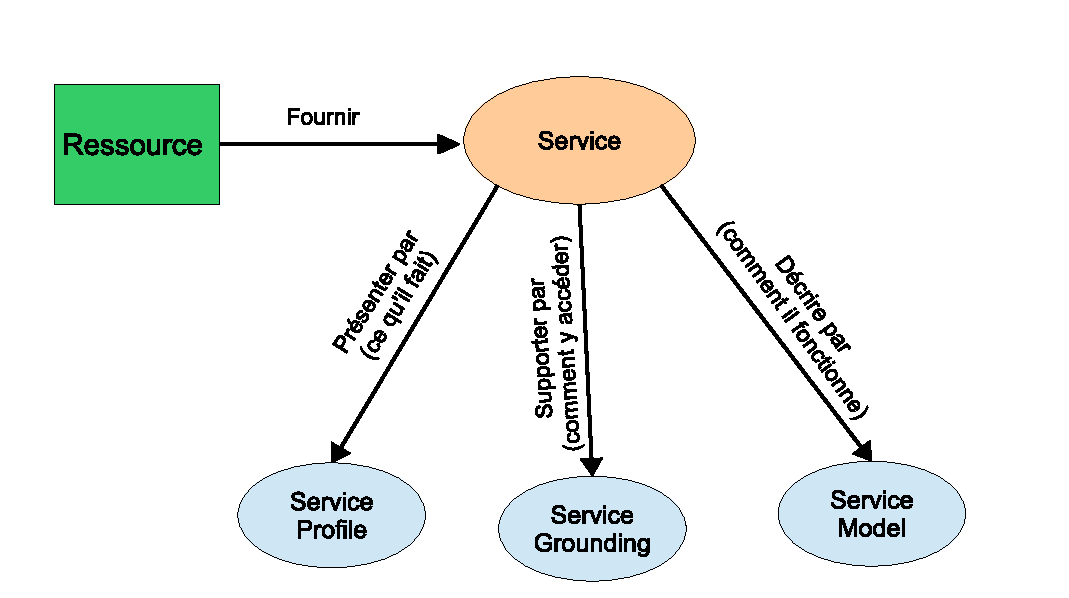
\includegraphics[width=0.8\textwidth]{figs/owls.eps}
    \caption{Les éléments d'une ontologie \textsc{OWL-S}}
    \label{fig:owl-s}
\end{figure}
 %TODO go for Tikz ✓

      L'objectif principal de ces recherches est d'établir une plateforme
      dans laquelle les descriptions des services Web sont partagés en
      utilisant une ontologie standard, constituée d'un ensembles de classes
      de base et des propriétés pour résoudre les ambigüités et de rendre la
      description d'un service compréhensible par une machine.

      la figure \ref{fig:owl-s} décrit la structure tripartie d'une
      ontologie \textsc{OWL-S}. Elle est composé de trois sous-ontologie: un
      \emph{service profile}, d'un \emph{service grounding} et d'un
      \emph{process model}.
      % TODO explain the fig:owl-s and add details about owls sub-ontologies
      \subsubsection{WSMO}
      \cite{baryannis2010}
      \newpage
  \section{Découverte des services web}
 % Description syntactique (UDDI) vs description sémantique

  % TOTANSLATE
  WS discovery is related to getting appropriate service for a
  request. It is one of the critical steps in the process of developing
  applications based on SOA. It can be done using syntactic matching or
  semantic matching\cite{Omer2011}.\\
  \newpage
  \section{Conclusion}
  % faire un petit récapitulatif sur les technologies des services web
  % rappeler de notre problème principale : composition des services web

%%% Local Variables: 
%%% mode: latex
%%% TeX-master: "../main"
%%% End: 
